\section{Sistema de comunicación}

Una vez habiamos creado el sistema de observaciones, quedaba que los agentes pudieran controlar a los jugadores del entorno. Pero para hacer esto surgía el mismo problema que con las observaciones, es necesario realizar una comunicacion entre el proceso de Python y el videojuego.

La primera idea que apareció fue usar una tecnologia de comunicacion actual, en concreto RabbitMQ \cite {RabbitMQ}. Esta es una tecnologia de para compartir mensajes entre procesos usando colas. Pero esta alternativa fue descartada rapidamente ya que no existe cliente de RabbitMQ en para Lua e implementar un cliente para esta plataforma requeriría mucho tiempo además de estar fuera del alcance de este proyecto. Por lo tanto decidimos reutilizar la alternativa 1 del sistema de comunicacion. En este caso, esta alternativa si que era viable ya que el tamaño de los datos a enviar es mucho menor, eliminando casi totalmente el problema de saturar el socket.

Adaptando la alternativa 1 del sistema de comunicacion, el proceso quedaría de la siguiente manera. El proceso de Python crearía el proceso de Mari0. Ambos procesos a su vez crean un thread que se encarga de la comunicación. Estos threads son necesarios para no bloquear la ejecución de los procesos principales. Y estos threads establecen una comunicación entre ellos usando un socket donde el thread de Mari0 actua como servidor y el de Python como cliente. Finalmente usando este socket, el proceso de Python y el videojuego pueden comunicarse mediante mensajes. Una de las ventajas de este sistema de comunicacion es que lo reutilizaremos para obtener las recompensas de las acciones de los agentes. Podemos ver el esquema del sistema de comunicacion en la figura \ref {fig:alternativa-1-acc}. 

\begin{figure}[ht]
    \centering
    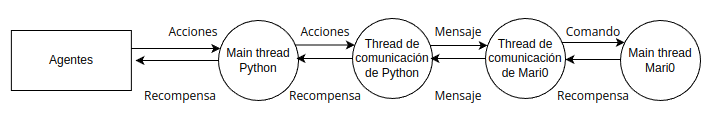
\includegraphics[width=1.0\textwidth]{img/comunication.png}
    \caption{Esquema de la alternativa por sockets[Elaboración Propia]}
    \label{fig:alternativa-1-acc}
\end{figure}


\subsection{Arquitectura de los mensajes}

La siguiente tarea era diseñar la arquitectura de los mensajes entre los procesos. Puesto que uno de nuestros objetivos era que el entorno fuera facilmente adaptable, necesitabamos crear una arquitectura de mensajes facilmente ampliable usando el paradigma de orientación a objetos. Partiendo de la base que cada agente puede ejecutar varias acciones o comandos en un mismo momento, decidimos crear la clase comando en Python.

Esta clase contendría el nombre del comando a ejecutar y los parametros necesarios para poder ejecutarlo correctamente. A partir de esta clase creamos una jerarquia de clases. La jerarquia se divide en comandos de juego y comandos de control. Los comandos de juego se componen de los comandos que pueden ejecutar los agentes, como saltar, disparar un portal, etc. Los comandos de control se componen de las diferentes acciones que se deben aplicar para gestionar el videojuego desde el proceso de Python. En concreto son las acciones de inicializar el mapa, resetear el entorno, obtener las recompensas, cerrar el juego y observar si se ha acabado el mapa. Como podemos deducir, los comandos de recompensa y de evaluar si se ha acabado el mapa requieren que el juego envie una respuesta. Por esto, tienen el atributo de need \_response. En Lua, decidimos crear la misma jerarquia de comandos que en Python, añadiendo además la operación Run() para implementar el funcionamiento de cada comando. En la figura \ref {fig:clases} podemos observar el esquema de la jerarquia de comandos.

\begin{figure}[ht]
    \centering
    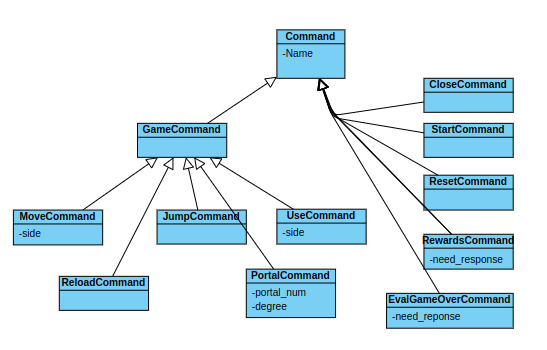
\includegraphics[width=1.0\textwidth]{img/clases.png}
    \caption{Esquema de las clases implementadas [Elaboración Propia]}
    \label{fig:clases}
\end{figure}

Adicionalmente, para facilitar el uso de estas clases, implementamos el patron Factory, para poder obtener a partir de la lista de acciones de un agente una lista de comandos. Una vez creados los comandos, enviamos el con los comandos en formato JSON al videojuego. Finalmente, una vez recibido el mensaje, el videojuego lo transforma de nuevo a una lista de comandos usando el modulo de JSON y de nuevo el patron Factory y ejecuta cada comando. Podemos ver un esquema de la secuencia de operaciones en la figura \ref {fig:operations}

\begin{figure}[ht]
    \centering
    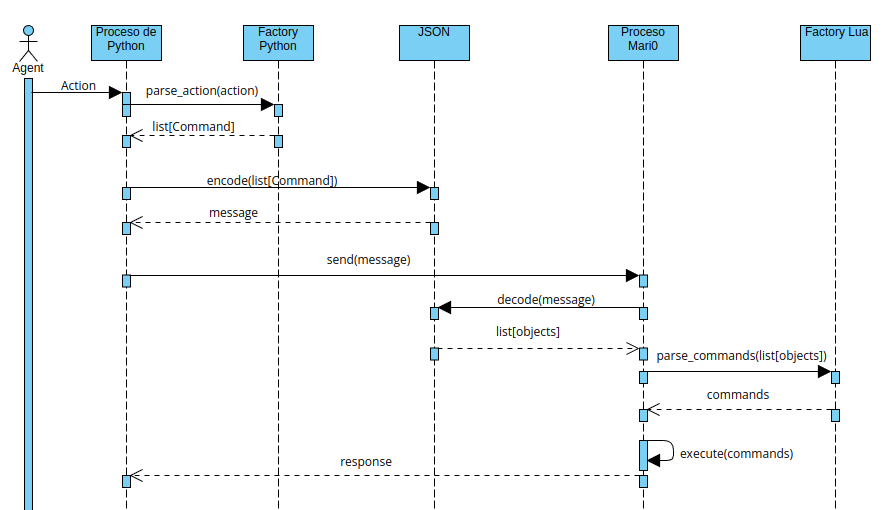
\includegraphics[width=1.0\textwidth]{img/secuencia_op.png}
    \caption{Esquema simplificado de la secuencia de operaciones en la comunicacion de comandos [Elaboración Propia]}
    \label{fig:operations}
\end{figure}

Una caracteristica a tener en consideración es que en caso que el proceso de Python envie un comando que requiere de respuesta, se quedará esperando a la respuesta del videojuego.

\subsection{Comunicación entre threads}

Otro aspecto que tuvimos que tener en cuenta fue la comunicacion entre los threads. Esta comunicacion se realizo en Python usando la clase cola. En concreto se crearon dos colas, una para enviar mensajes y otra para recibir las respuestas del videojuego. De forma paralela, en Lua se usaron 2 canales, que son identicos a las colas, uno para obtener los comandos a ejecutar y otro para enviar las respuestas al entorno. En la figura \ref {fig:threads} podemos ver el esquema de la comunicacion entre threads. 

\begin{figure}[ht]
    \centering
    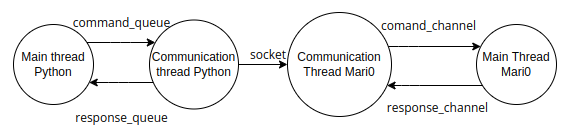
\includegraphics[width=1.0\textwidth]{img/threads.png}
    \caption{Esquema de la comunicacion entre threads [Elaboración Propia]}
    \label{fig:threads}
\end{figure}

\subsubsection*{Problemas encontrados}

Realizando la implementación la comunicación nos encontramos con varios problemas. En esta seccion explicaremos brevemente los problemas que tuvimos y su solucion.

\begin{itemize}
    \item Implementación de los comandos en el juego. De los mayores problemas que hubo fue conseguir que cada comando ejecutará la operación deseada, sobretodo el principal problema consistió en el movimiento. La solución fue debbugear el codigo.
    \item Bloqueo de los threads de comunicacion. Puesto que los threads de comunicacion deben coordinarse entre ellos para enviar mensajes a traves de los channels o las colas y a traves de los sockets, si no se gestionaba correctamente los threads se bloqueaban esperando mensajes. Para solucionar estos problemas se implemento un tiempo de espera maximo y en caso de no obtener el mensaje esperado se continuaria normalmente con la ejecución.
\end{itemize}